\clearpage
\section{Database structure}

The database consists of the following three tables, shown in fig. \ref{fig:DB_ER} 
\begin{itemize}
    \item user
    \item user\_role
    \item role
\end{itemize}

\begin{figure}[H]
    \centering
    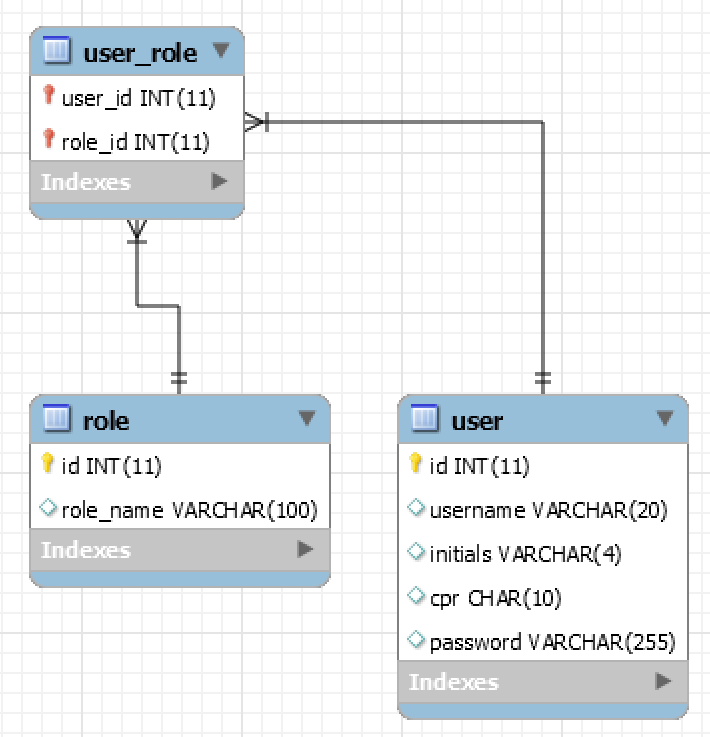
\includegraphics{diagrams/DB_ER_Diagram.PNG}
    \caption{Database Entity-Relationship diagram. See \ref{fig:DB_ER_legend} for symbol legend.}
    \label{fig:DB_ER}
    % This one taken from website, should get cited
    % https://www.lucidchart.com/pages/ER-diagram-symbols-and-meaning
\end{figure}

\begin{figure}[H]
    \centering
    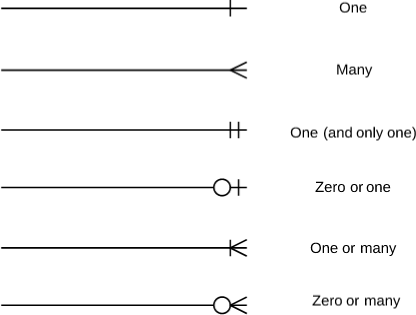
\includegraphics[width=0.5\linewidth]{diagrams/ERD_notation-416x315.PNG}
    \caption{Symbol explanation for fig. \ref{fig:DB_ER_legend}}
    \label{fig:DB_ER_legend}
\end{figure}

\noindent In user\_role table, two foreign keys marked with a red key, binding together the user table with the role table.
The yellow keys in both user and role tables are  the primary keys.There is a one (and only one) to many 
relationship between both user and role towards user\_role. The idea of having a table for both user and role is 
because a user can have more than one role. The unique ID for both user and role are added to user\_role, which then 
makes it easy to fetch all the roles one user has. 